\subsection{Average Focal Plane Reconstruction}
\label{avg_kidpar}

\noindent {\bf FM: Figures \ref{fig:avg_fov_color}, \ref{fig:jumping_kids} and \ref{fig:mean_vs_median} are too large.
captions cannot be read}
 

\begin{figure}[p]
\begin{center}
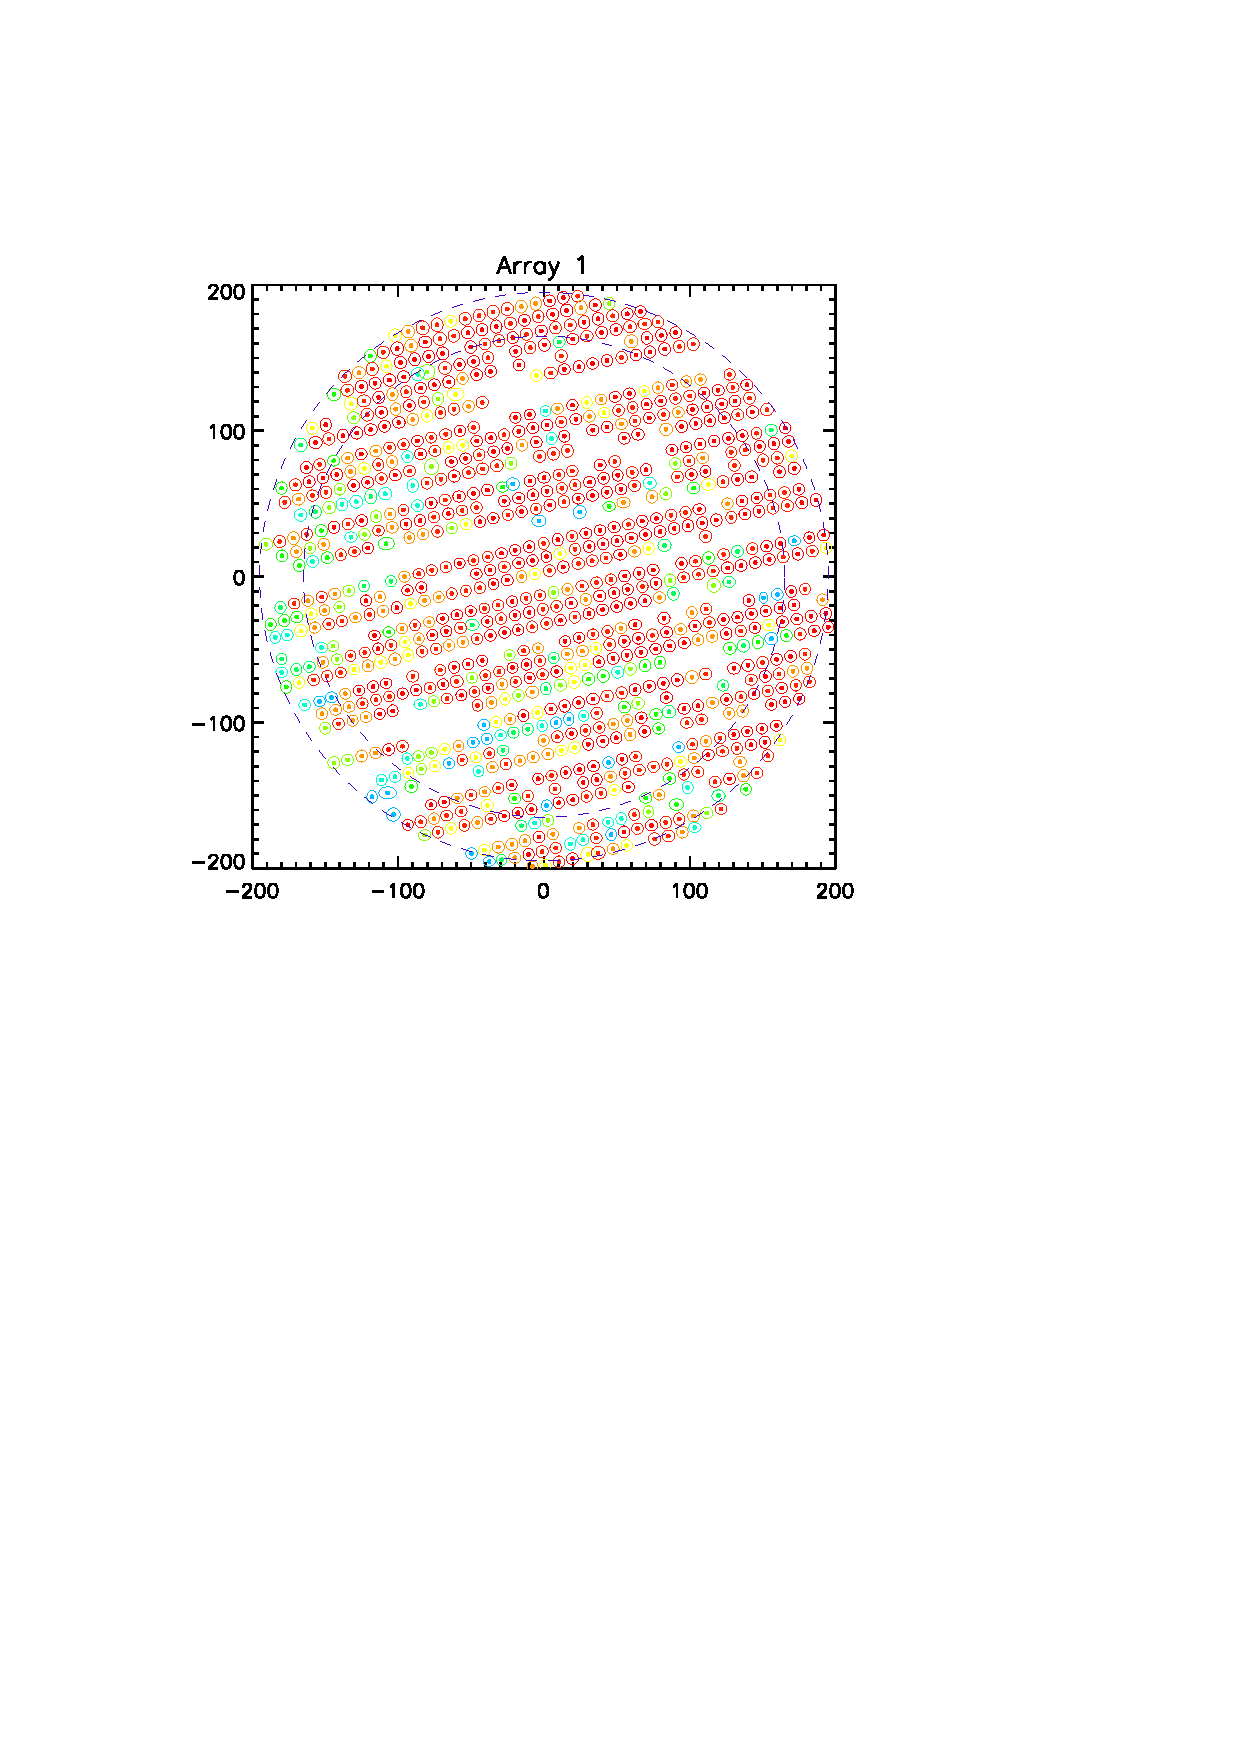
\includegraphics[trim=2cm 14cm 4cm 4cm, clip=true,width=0.6\linewidth]{Figures/A1_fwhm_color_count.pdf}
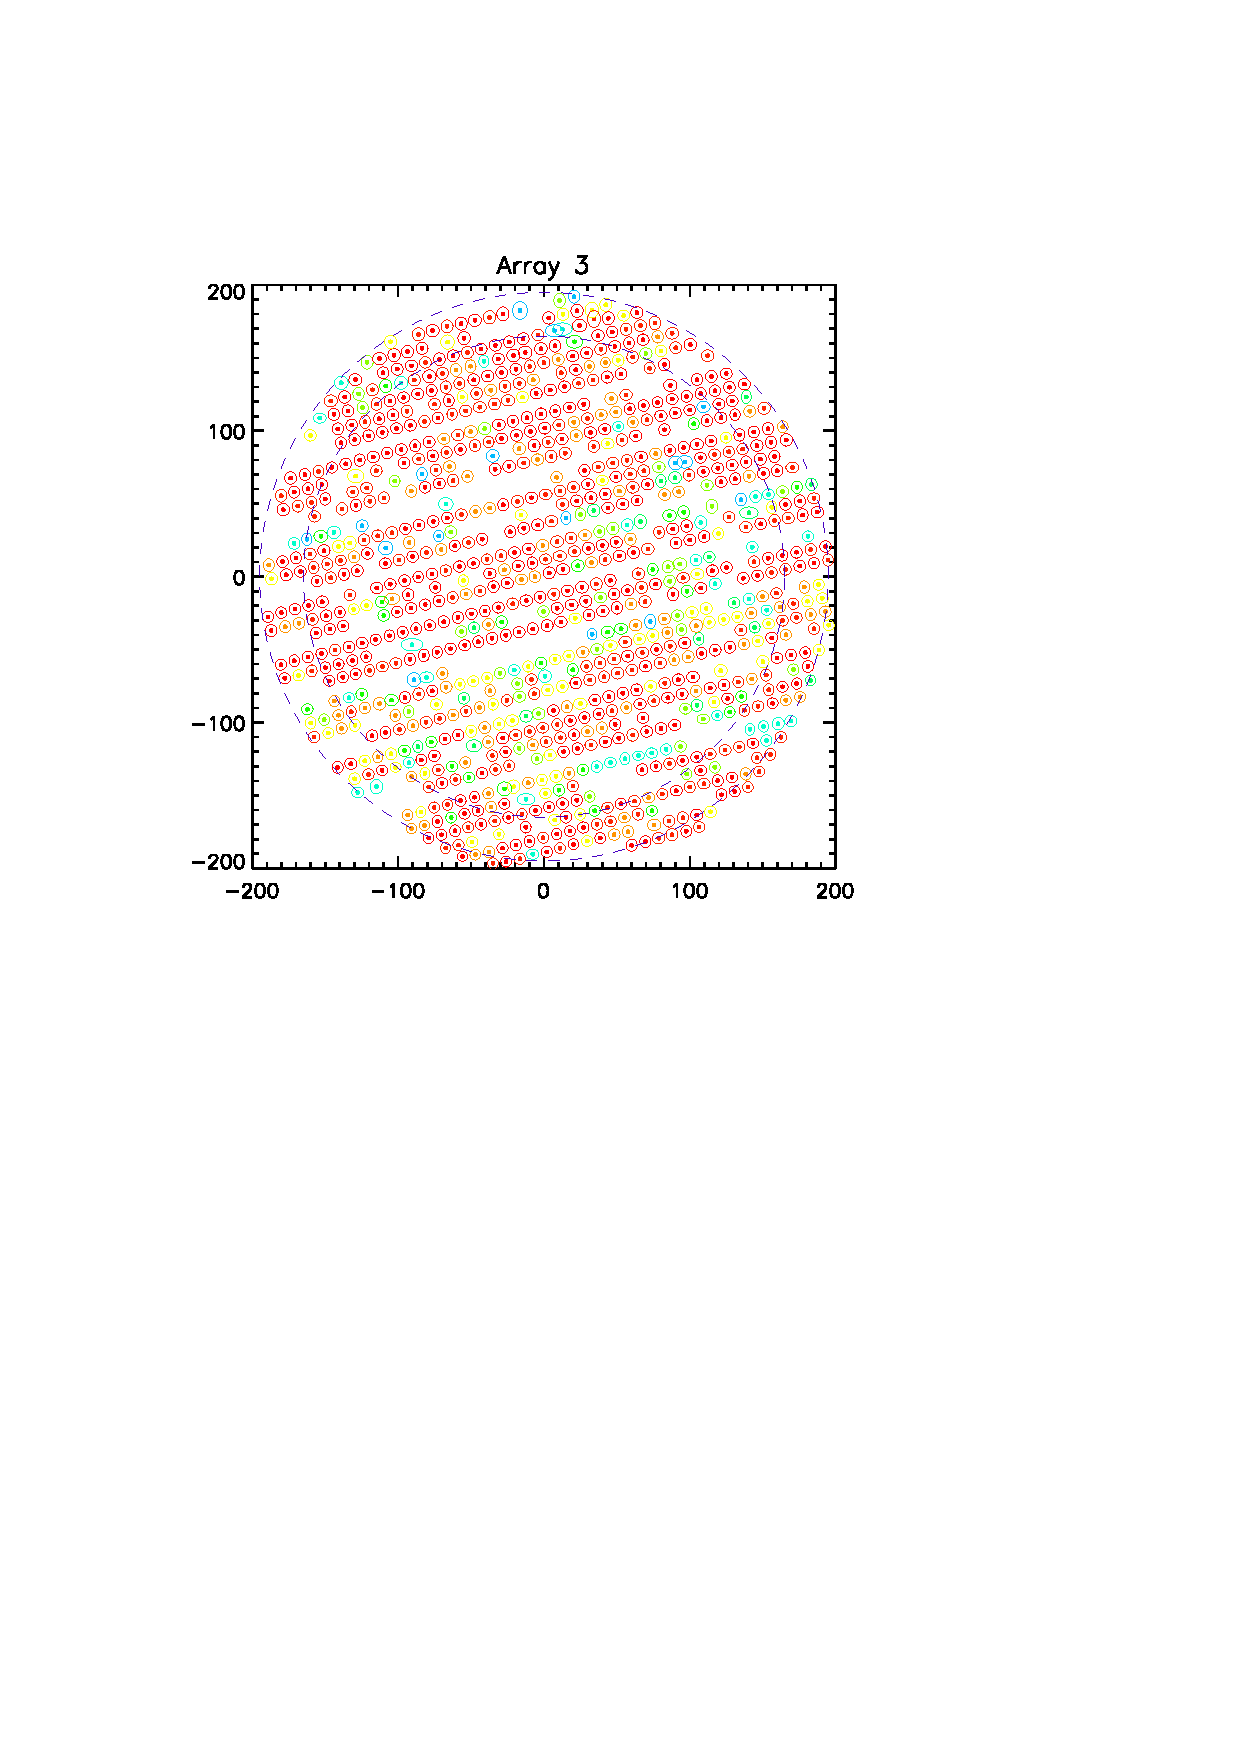
\includegraphics[trim=2cm 14cm 4cm 4cm, clip=true,width=0.6\linewidth]{Figures/A3_fwhm_color_count.pdf}
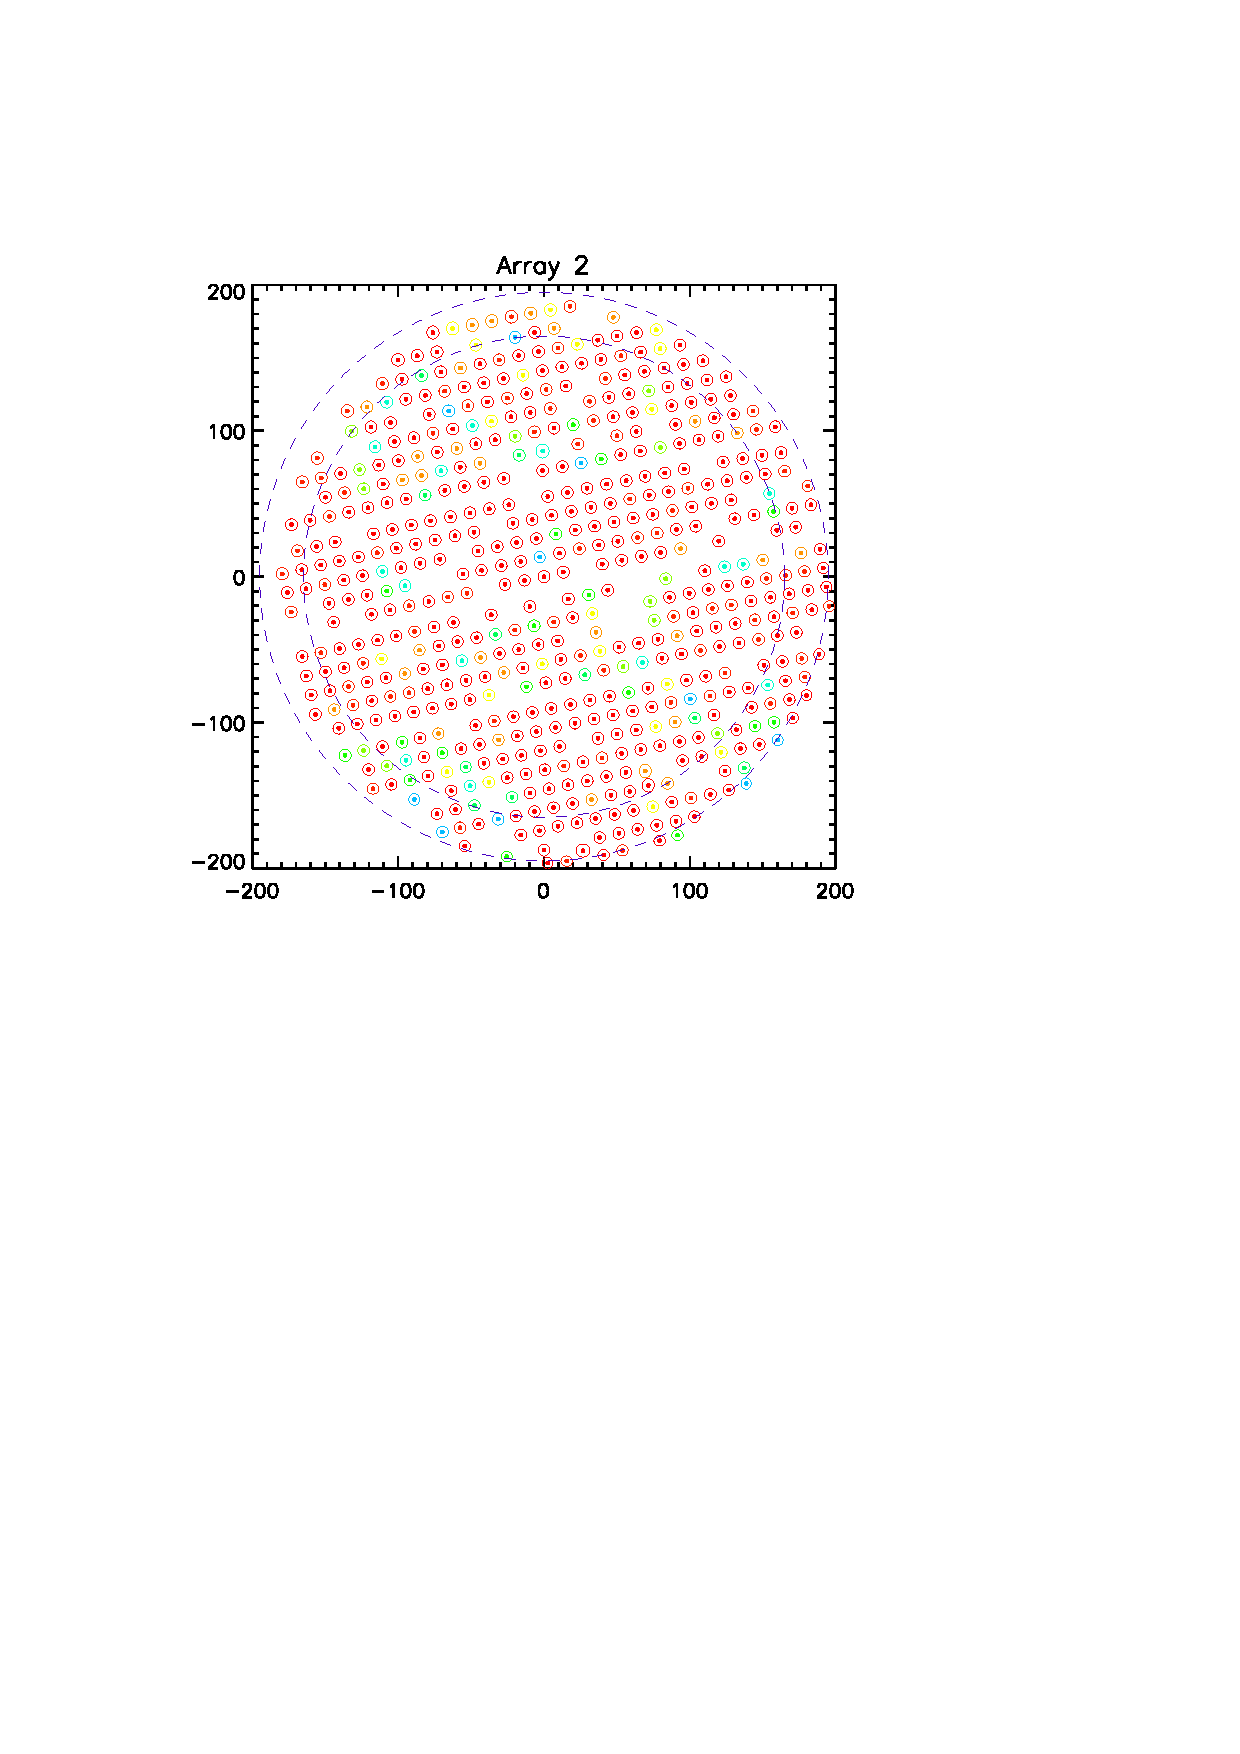
\includegraphics[trim=2cm 14cm 4cm 4cm, clip=true,width=0.6\linewidth]{Figures/A2_fwhm_color_count.pdf}
\caption{Average detectors positions for arrays A1, A3, and A2 (from
  green to red as a function of the number of times that a given pixel
  has been considered as valid). The three plots show the detectors
  that have seen the sky and passed the quality criteria for at least
  two beam maps during Run10, 9 and 8: 952, 961, and 553
  %925, 944, and 543
  for A1, A3 and A2, respectively. The inner and outer dash-line circles correspond to a 
  FOV of 5.5$\prime$ and 6.5$\prime$, respectively. Units are arcseconds. 
  The color (from green to red)  shows the number of times that a given pixel has been considered as valid.}
\label{fig:avg_fov_color}
\end{center}
\end{figure}

In order to identify the most stable pixels, we compare the KIDs parameter obtained with several beam maps. 
In the following, we   show results as obtained using seven beam maps from Run10, two from Run9 and one from Run8.
For each pixel we compute the average position on the focal plane and the average FWHM, counting the times that it has been considered as valid.

In Fig. \ref{fig:avg_fov_color} we show the average focal plane
reconstruction, from green to red depending on the number of times
that the pixel has been considered as valid. For A1, A3 and A2,
respectively, we have 952, 961, and 553 pixels that have been
considered as valid at least twice (840, 508, 868 valid at least five
times).
% LP: add a sentence to reference Table ``\ref{tab:number_of_kids}"
Using this criterion, we deduce the fraction of valid
detectors over the designed ones, as given in Table~\ref{tab:number_of_kids}. 
As a second step, we also flag pixels that move across the focal plane from a 
beam map to another (Fig. \ref{fig:jumping_kids} , jumping KIDs) and those 
who share the same position (twin KIDs). To identify the former, we look at the difference 
of the mean and median position of each KID (the red crosses and black squares in 
Fig. \ref{fig:mean_vs_median}). For the latter a criterion on the position is applied in 
order to find the pixels that are closer than the grid step.

\begin{figure}[htp]
\begin{center}
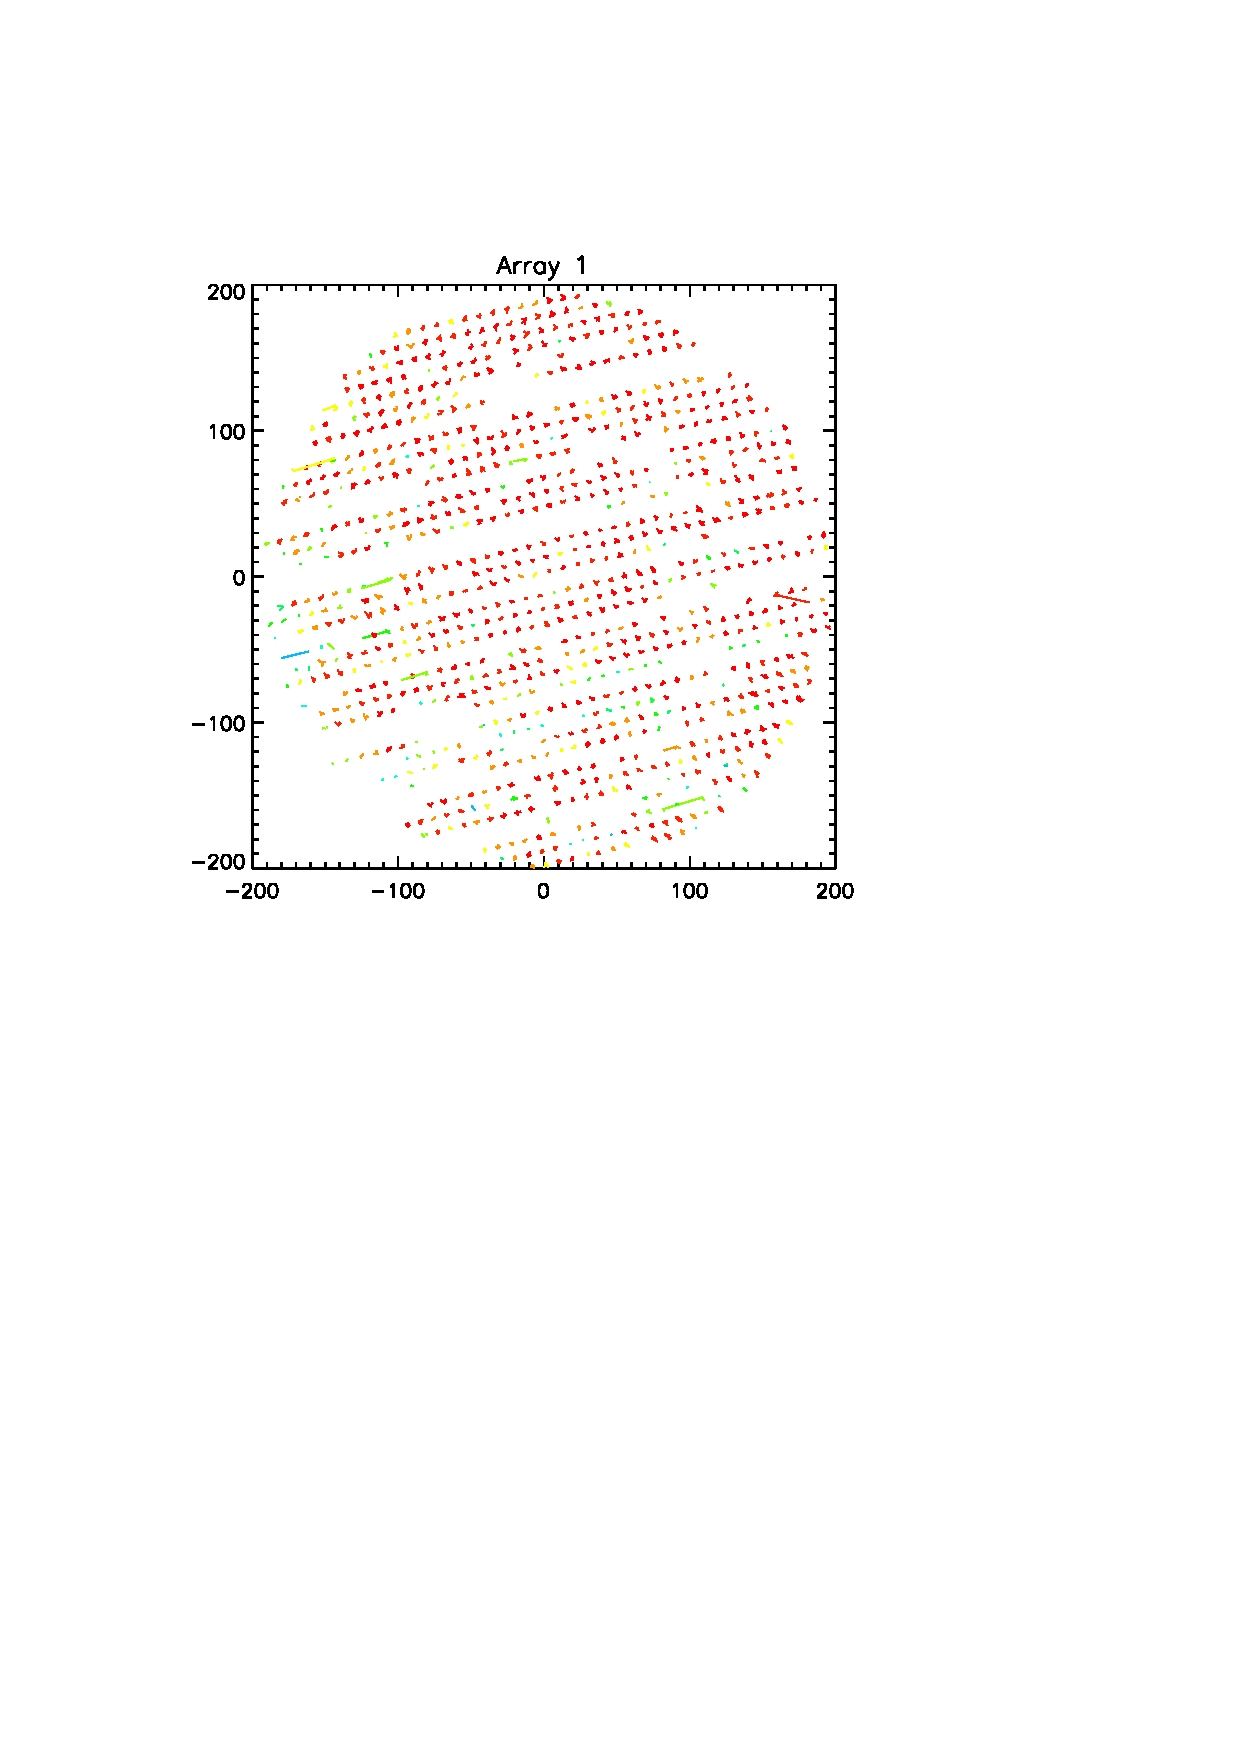
\includegraphics[trim=2cm 14cm 5cm 4cm, clip=true,width=0.6\linewidth]{Figures/A1_positions.pdf}
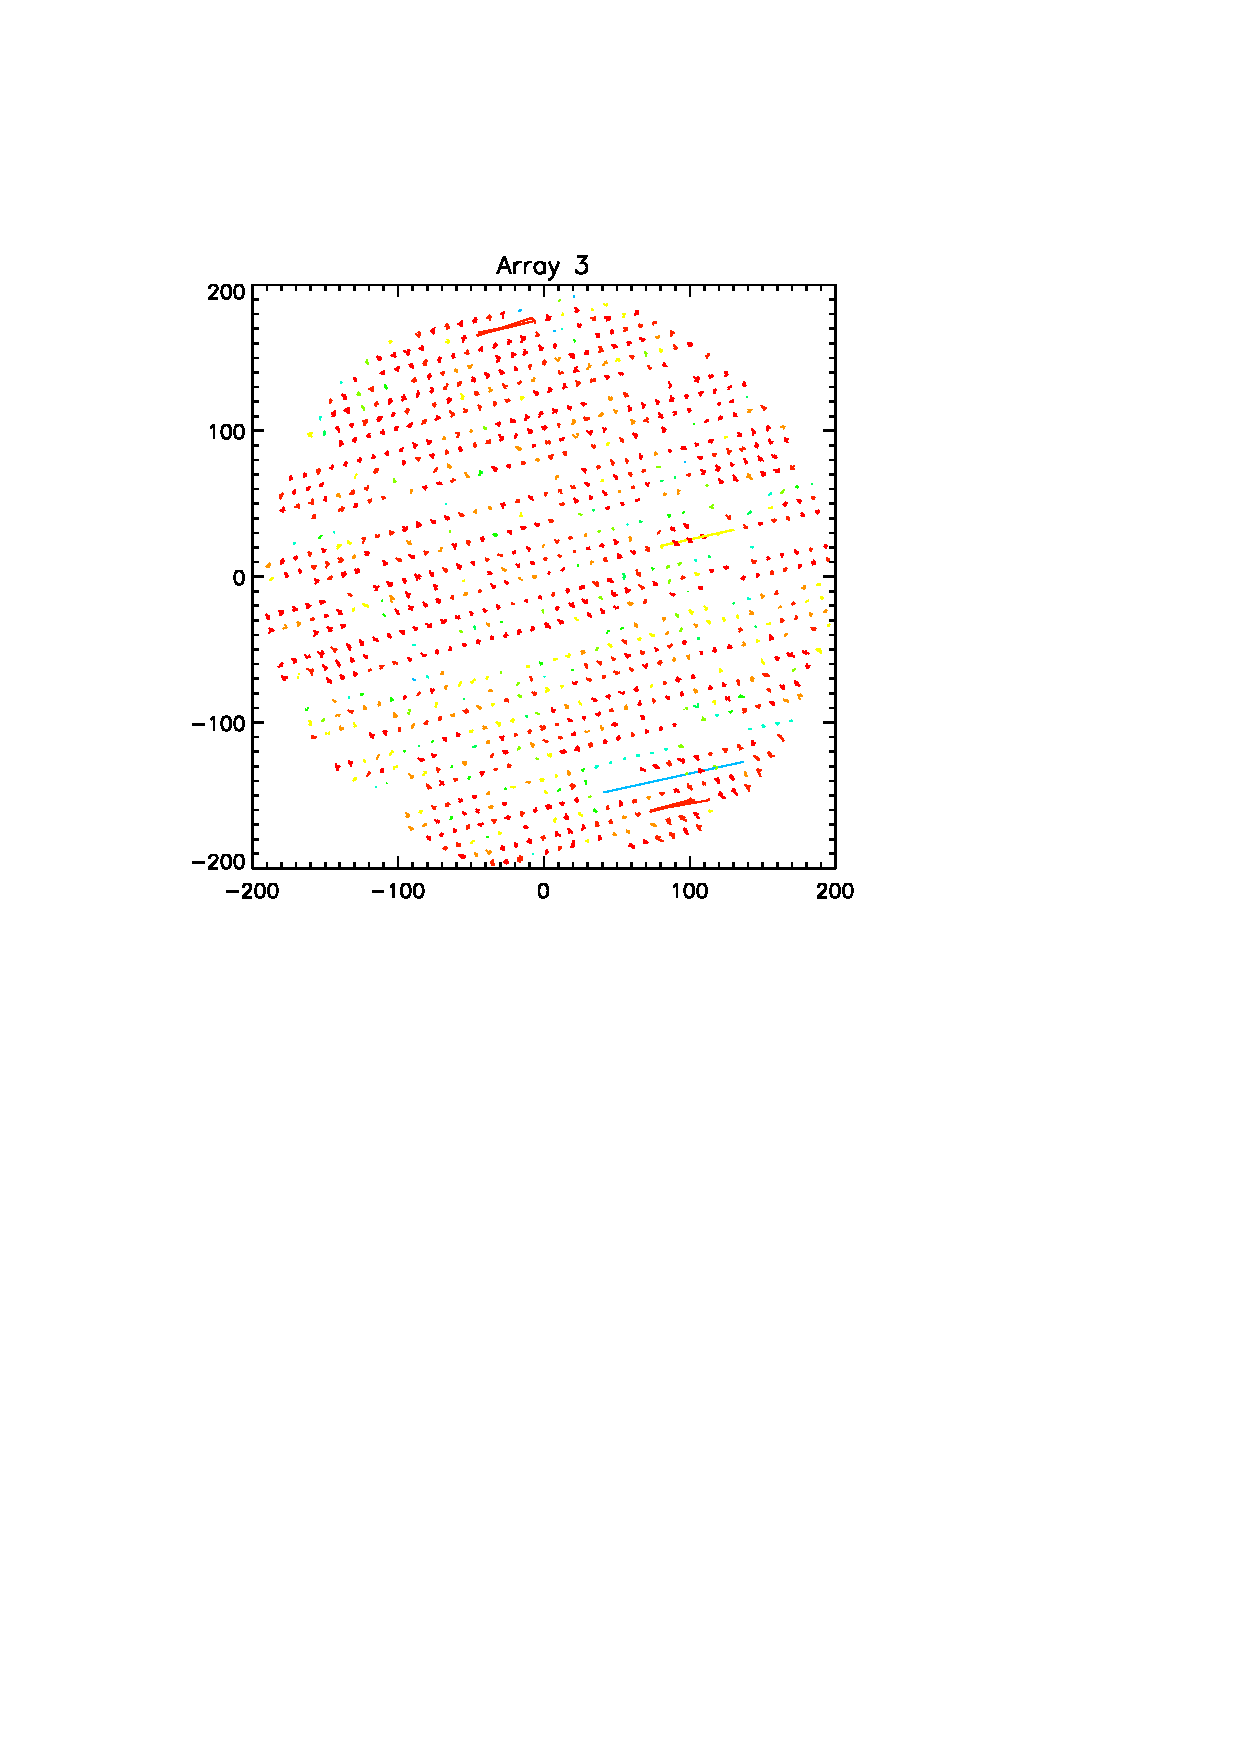
\includegraphics[trim=2cm 14cm 5cm 4cm, clip=true,width=0.6\linewidth]{Figures/A3_positions.pdf}
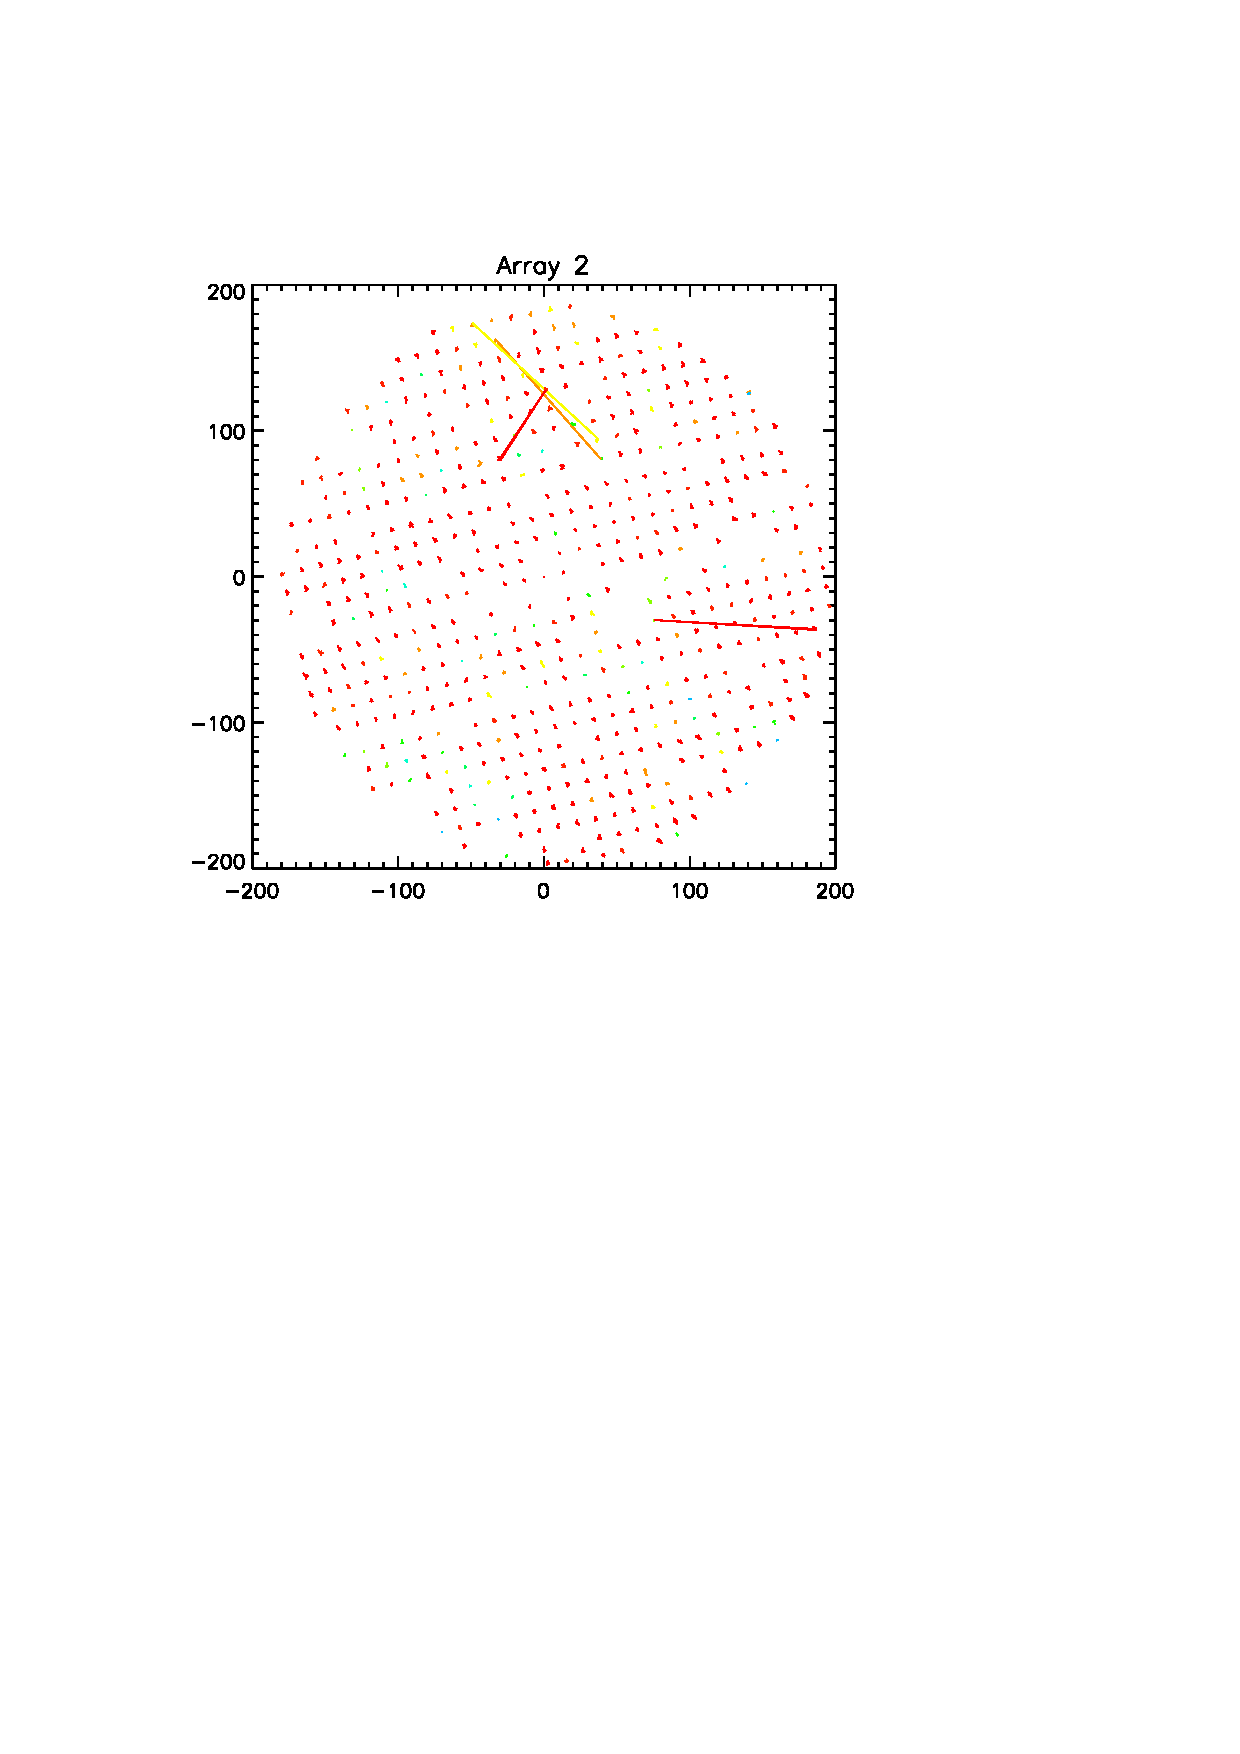
\includegraphics[trim=2cm 14cm 5cm 4cm, clip=true,width=0.6\linewidth]{Figures/A2_positions.pdf}
\caption{For the 952, 961, and 553 pixels that have passed the quality criteria at least twice for A1, A3 and A2, we show the positions of each pixel, as obtained from each beam map. We can see that some of them are not found at the same position for all the beam maps. Units are arcseconds.}
\label{fig:jumping_kids}
\end{center}
\end{figure}

\begin{figure}[htp]
\begin{center}
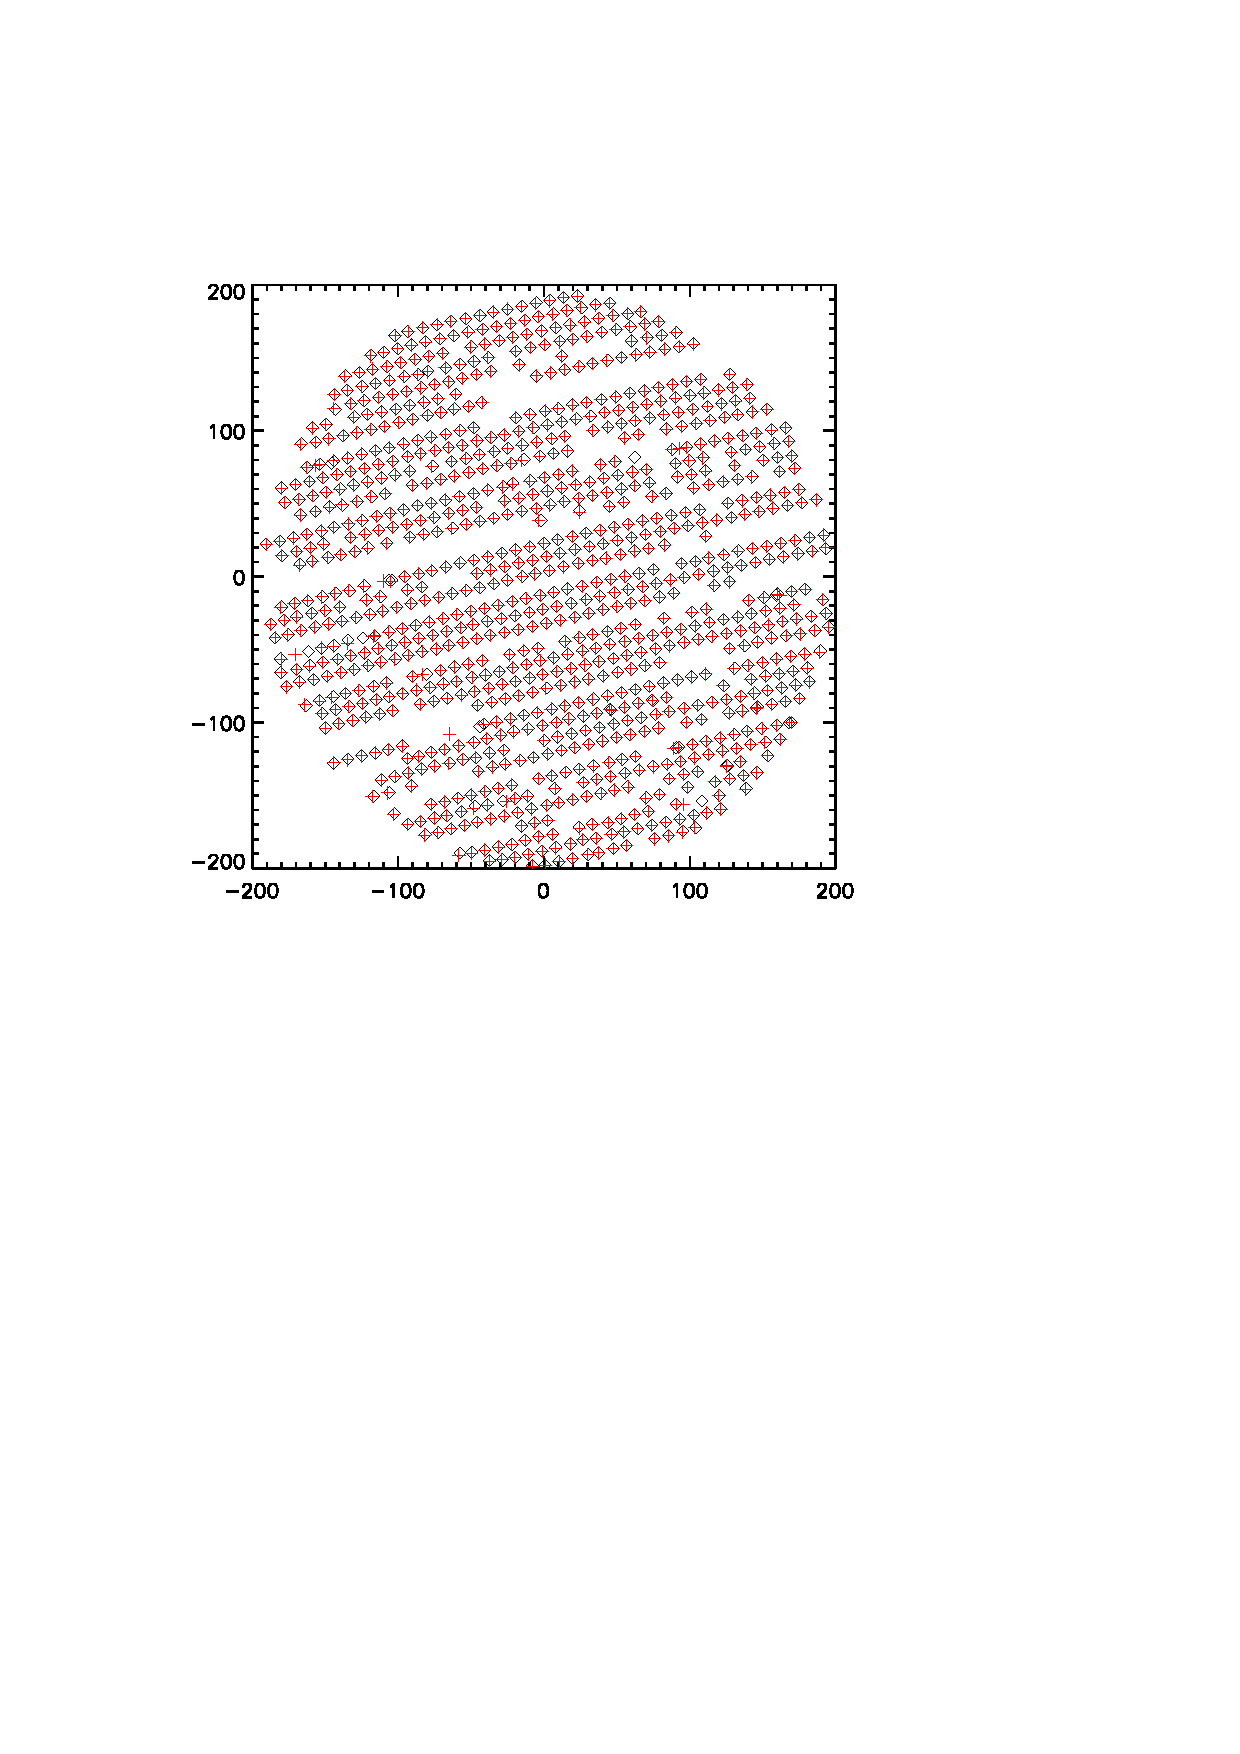
\includegraphics[trim=2cm 14cm 5cm 4cm, clip=true,width=0.6\linewidth]{Figures/A1_test_positions.pdf}
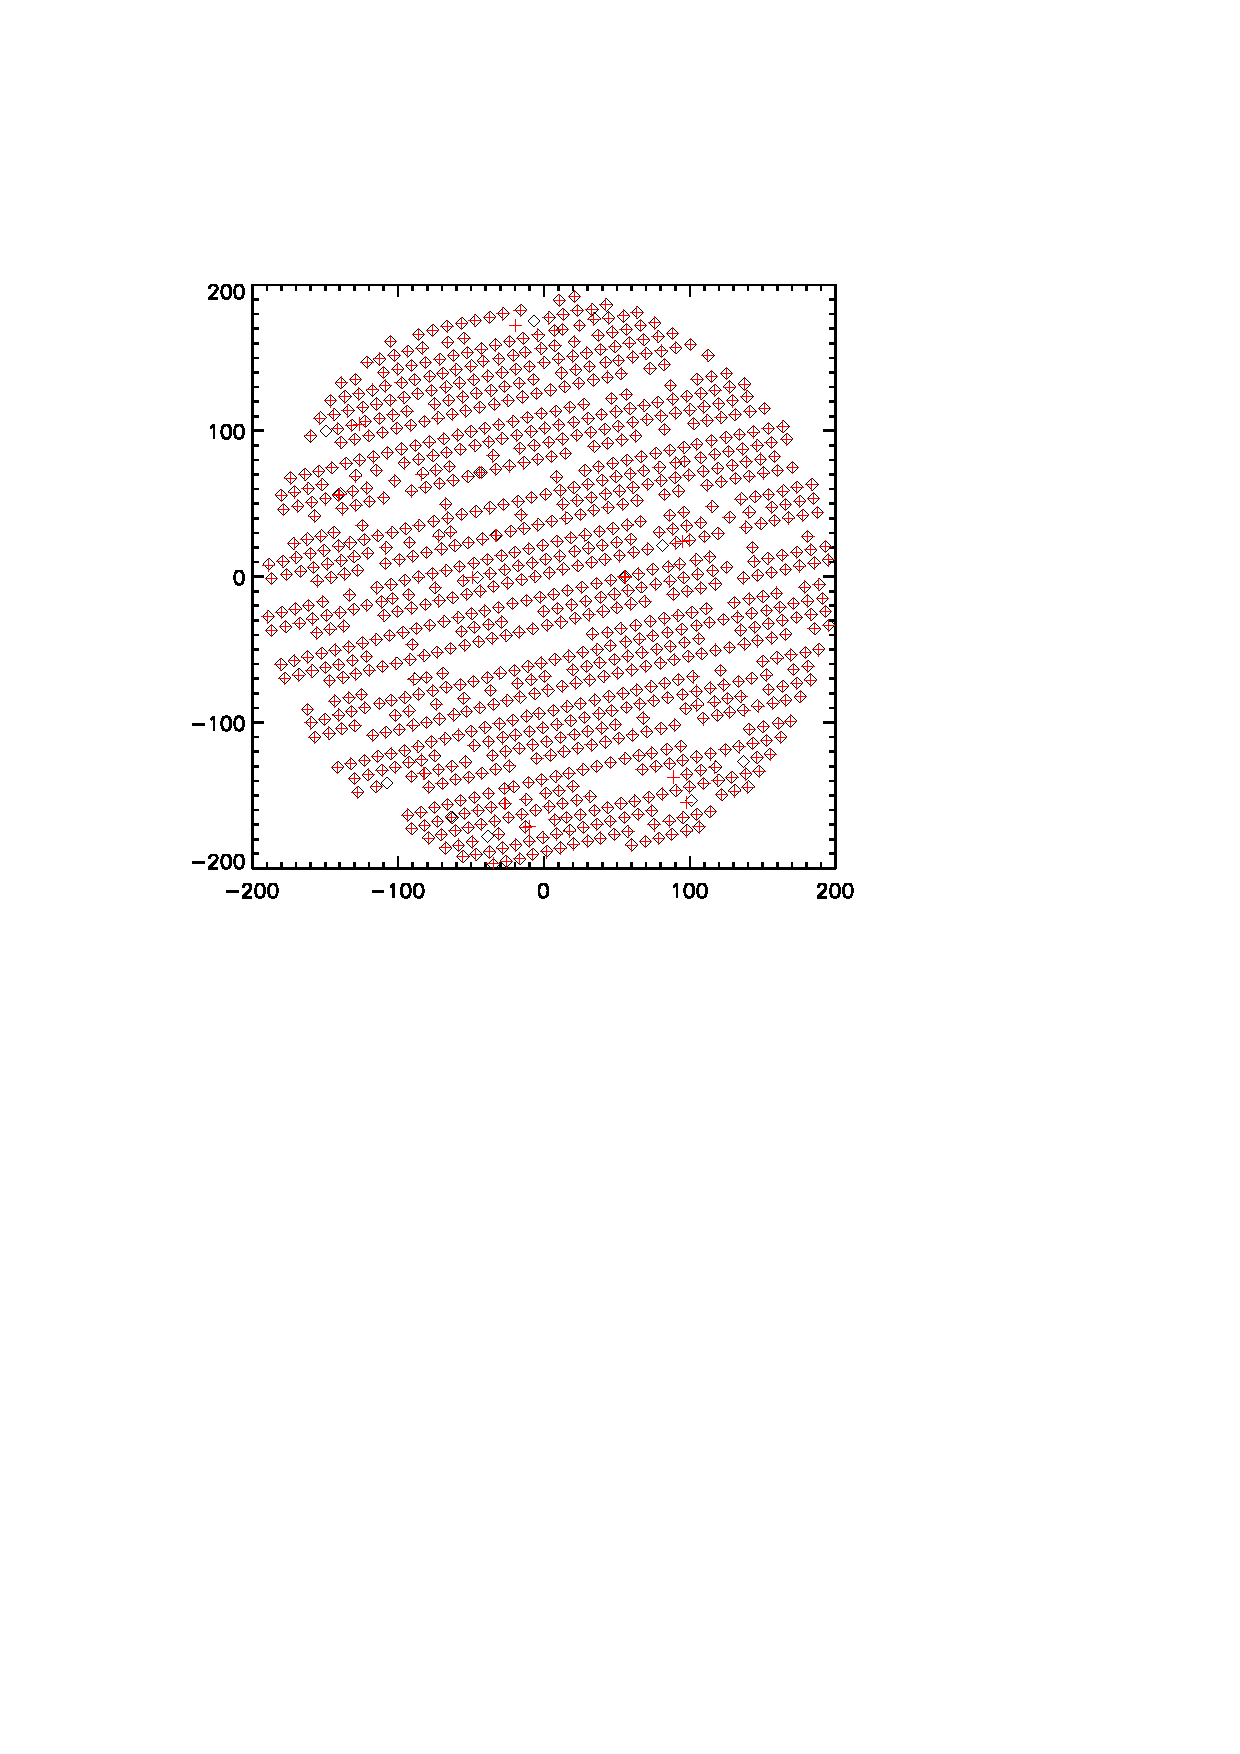
\includegraphics[trim=2cm 14cm 5cm 4cm, clip=true,width=0.6\linewidth]{Figures/A3_test_positions.pdf}
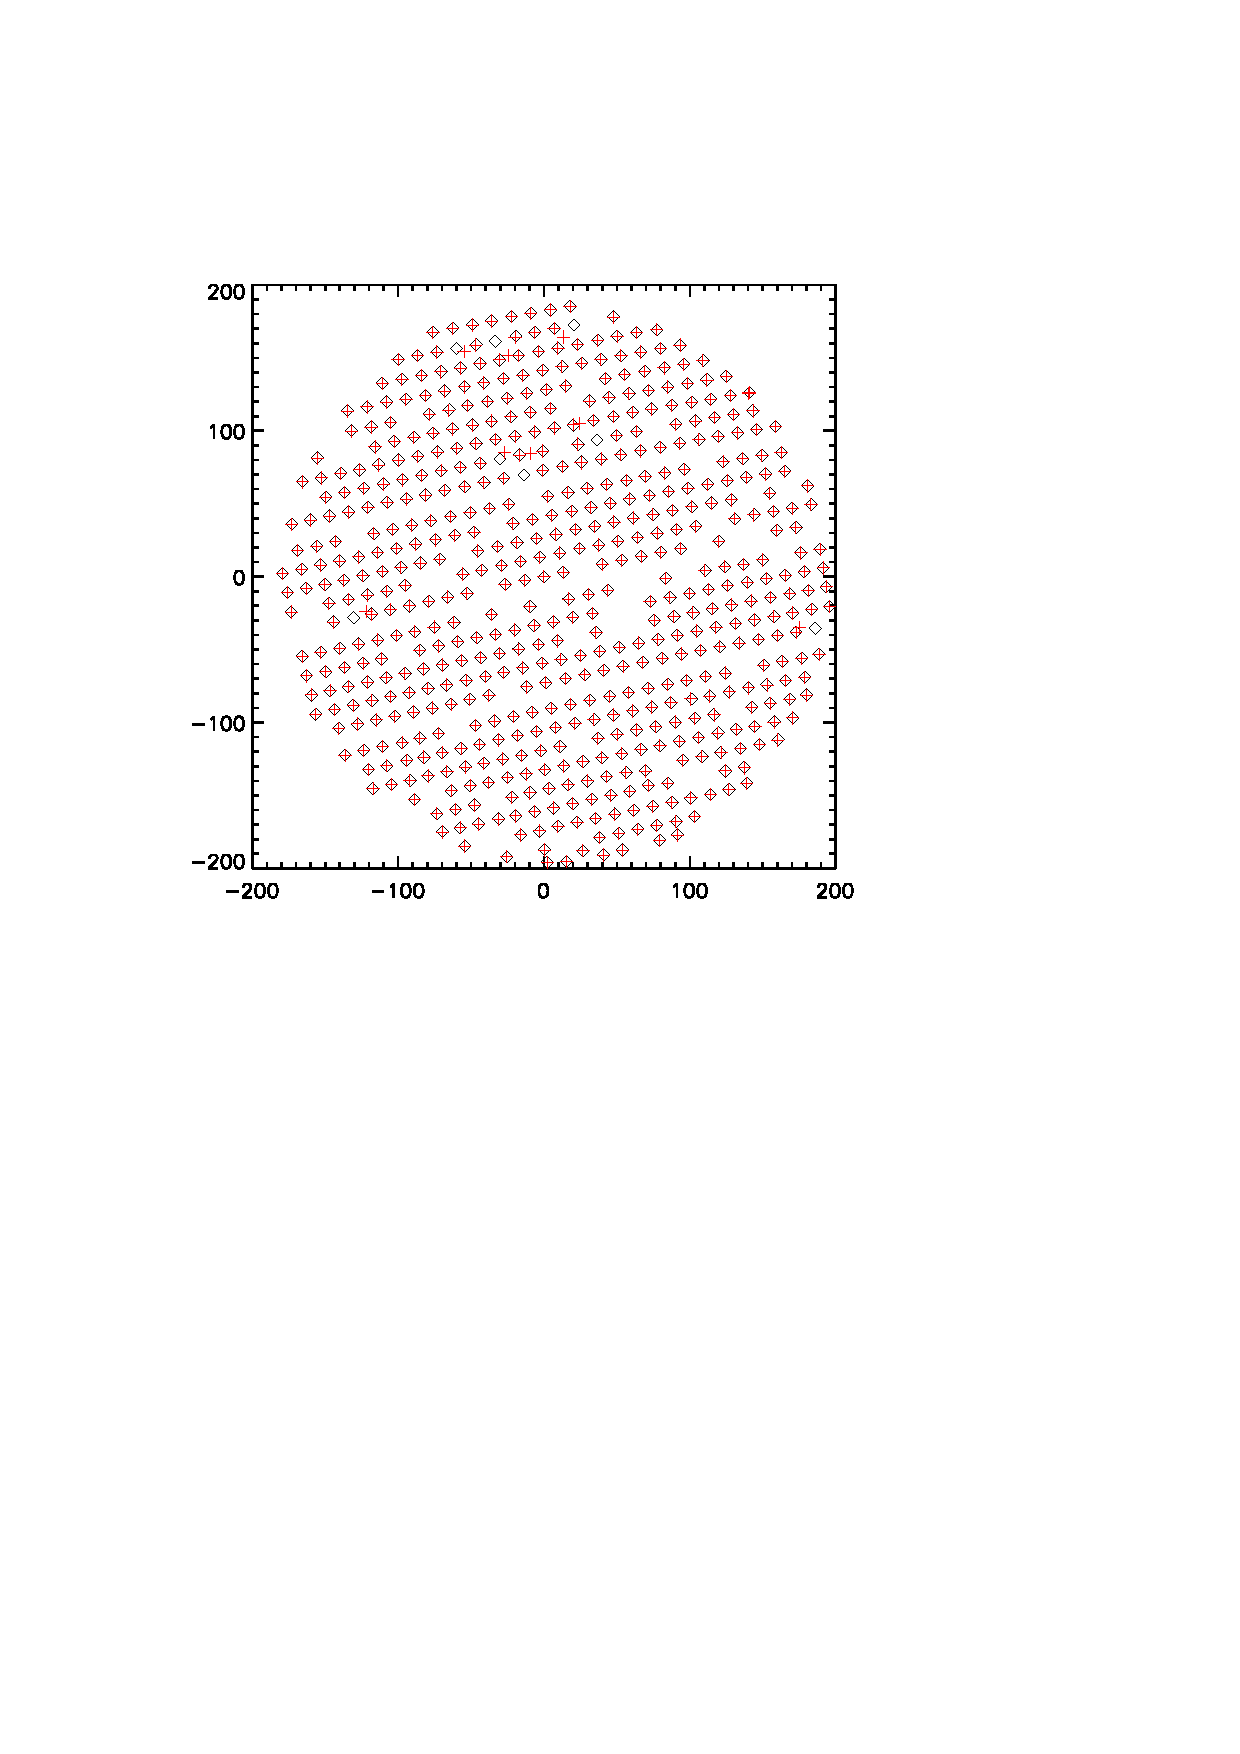
\includegraphics[trim=2cm 14cm 5cm 4cm, clip=true,width=0.6\linewidth]{Figures/A2_test_positions.pdf}
\caption{For the 952, 961, and 553 pixels that
  have passed the quality criteria at least twice for A1, A3 and A2,
  we show the mean (red crosses) and the median (black squares)
  positions of each pixel, as obtained from each beam map.
  Units are arcseconds. }
\label{fig:mean_vs_median}
\end{center}
\end{figure}


% LP: copy from fov.tex + modif according to Samuel's comment
\begin{table}[ht]
\begin{center}  
  \begin{tabular}{|c|c|c|c|}
    \hline
    Array & Designed detectors &  Valid detectors & Fraction\\
    \hline\hline
    A1 & 1140 & 952 &  84\%\\
    A3 & 1140 & 961 &  84\%\\
    A2 & 616  & 553 &  90\%\\
    \hline
  \end{tabular}
  \caption{ CAPTION}
  \label{tab:number_of_kids}
\end{center}    
\end{table}
